\documentclass{beamer}
\usepackage[latin1]{inputenc}
%\usetheme[noshadow,nonav,nologo]{NYU}
\usetheme[numbers]{NYU}
\usepackage{amsmath}
\usepackage{amsfonts}
\usepackage{amssymb}
\usepackage{color, colortbl}
\usepackage{graphicx}
\usepackage{subfigure}
\usepackage{caption}
\usepackage{lmodern}
\usepackage{subcaption}
\usepackage{epstopdf}


\makeatletter
\newcommand{\thickhline}{%
    \noalign {\ifnum 0=`}\fi \hrule height 2pt
    \futurelet \reserved@a \@xhline}

\title{Unsupervised Learning of Deep Feature Hierarchies from Unlabeled Video Data}
\date{ \tiny Courant Institute of Mathematical Sciences \\ \vspace{0.33cm} \tiny September 2015} 
\author{Ross Goroshin}

\begin{document}
\begin{frame}
\titlepage
\end{frame}

\begin{frame}
\begin{columns}[T] % align columns
\begin{column}{.33\textwidth}
\color{blue}\rule{\linewidth}{2pt}
\tiny{Visibility Path Planning via Variational Optimization }
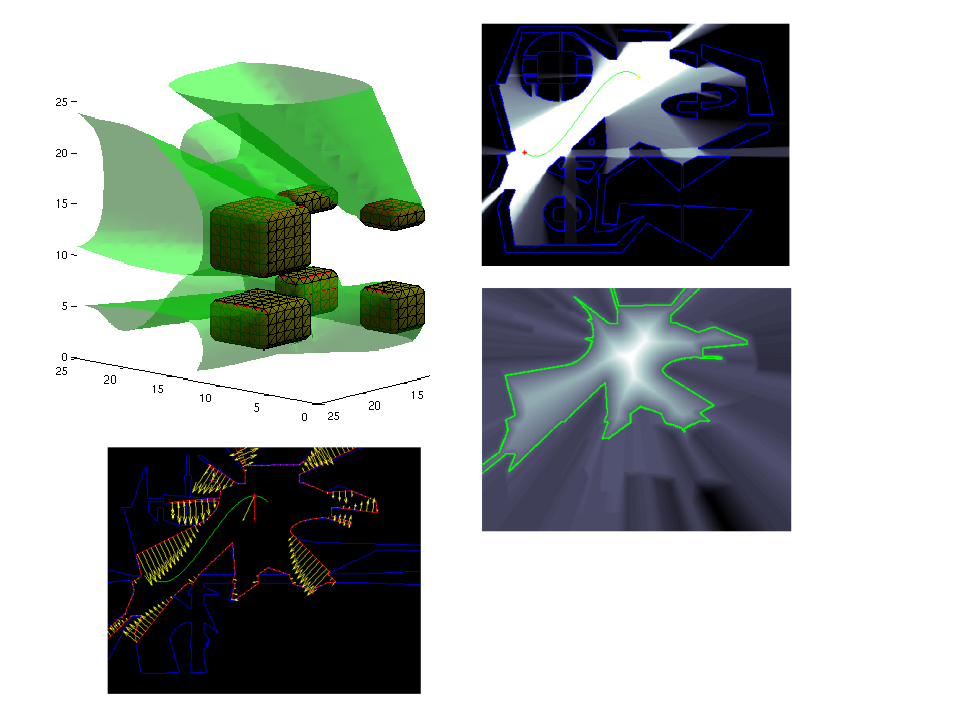
\includegraphics[scale=0.3,trim = 1 30 1 1, clip]{./Figures/vis.pdf}
\end{column}%
\hfill%
\begin{column}{.33\textwidth}
\color{blue}\rule{\linewidth}{2pt}
\tiny{Cable Detection in Sonar Imagery}
\centering
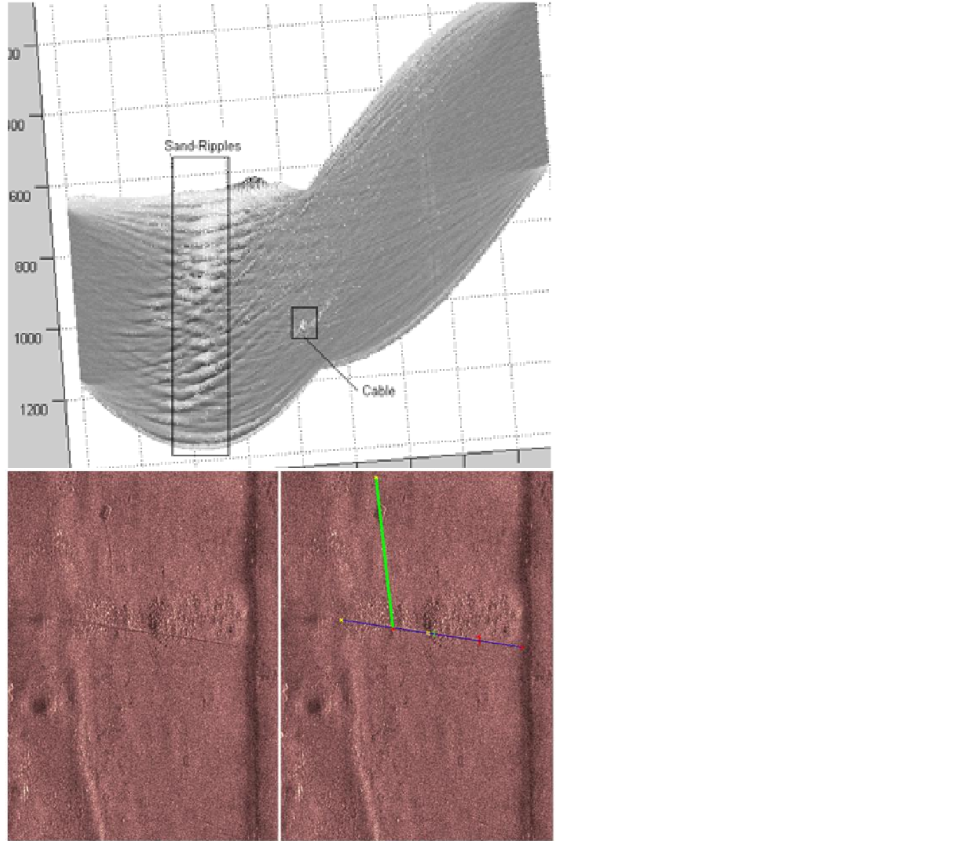
\includegraphics[scale=0.30,trim = 1 1 200 40, clip]{./Figures/cable.pdf}
\end{column}%
\begin{column}{.33\textwidth}
\color{blue}\rule{\linewidth}{2pt}
\tiny{Segmentation with Active-Contours}
\centering
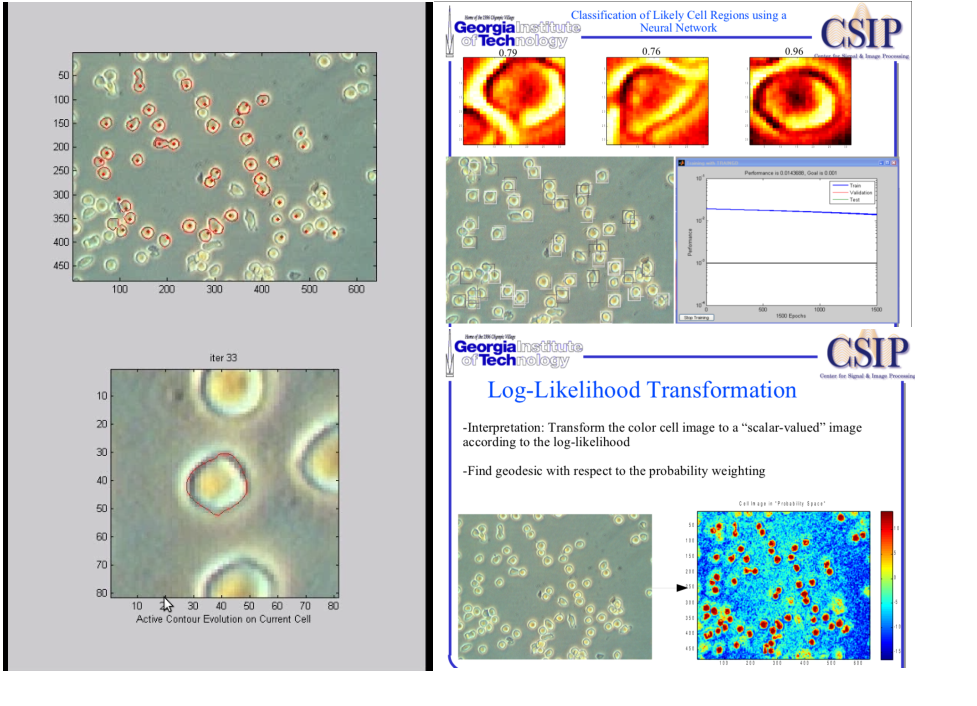
\includegraphics[scale=0.35,trim = 1 1 260 10, clip]{./Figures/cells.pdf}
\end{column}%
\end{columns}
\vspace{0.5cm} 
\begin{columns}[T] % align columns
\begin{column}{.48\textwidth}
\color{blue}\rule{\linewidth}{2pt}
\tiny{Monocular Obstacle Detection}
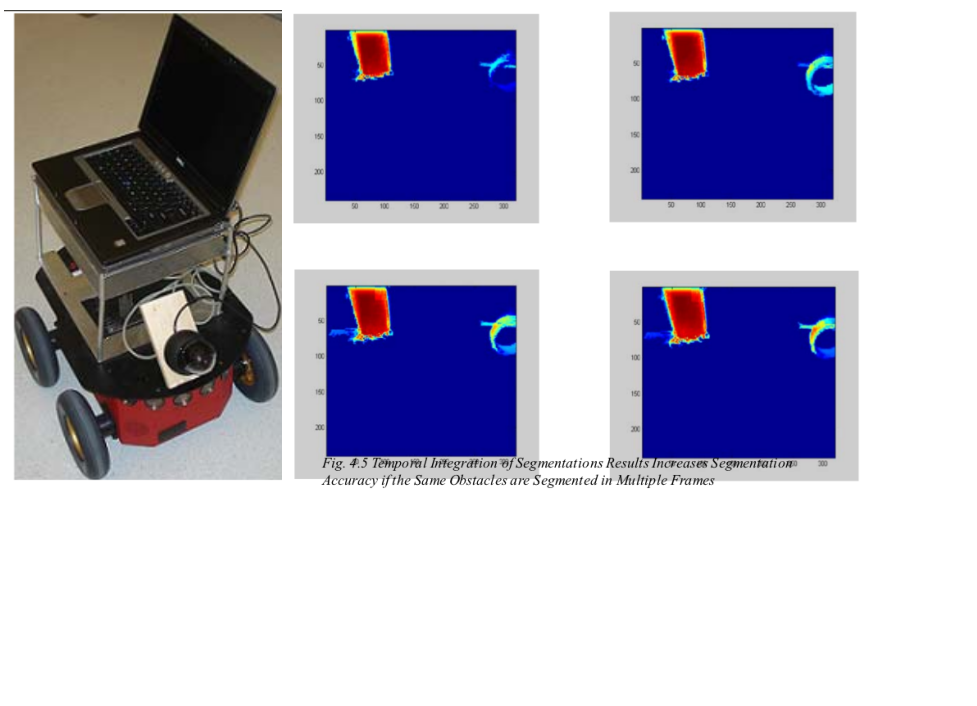
\includegraphics[scale=0.40,trim = 1 1 30 10, clip]{./Figures/obs.pdf}
\end{column}%
\hfill%
\begin{column}{.48\textwidth}
\color{blue}\rule{\linewidth}{2pt}
\tiny{Synthetic Aperture Sonar Imaging}
\centering
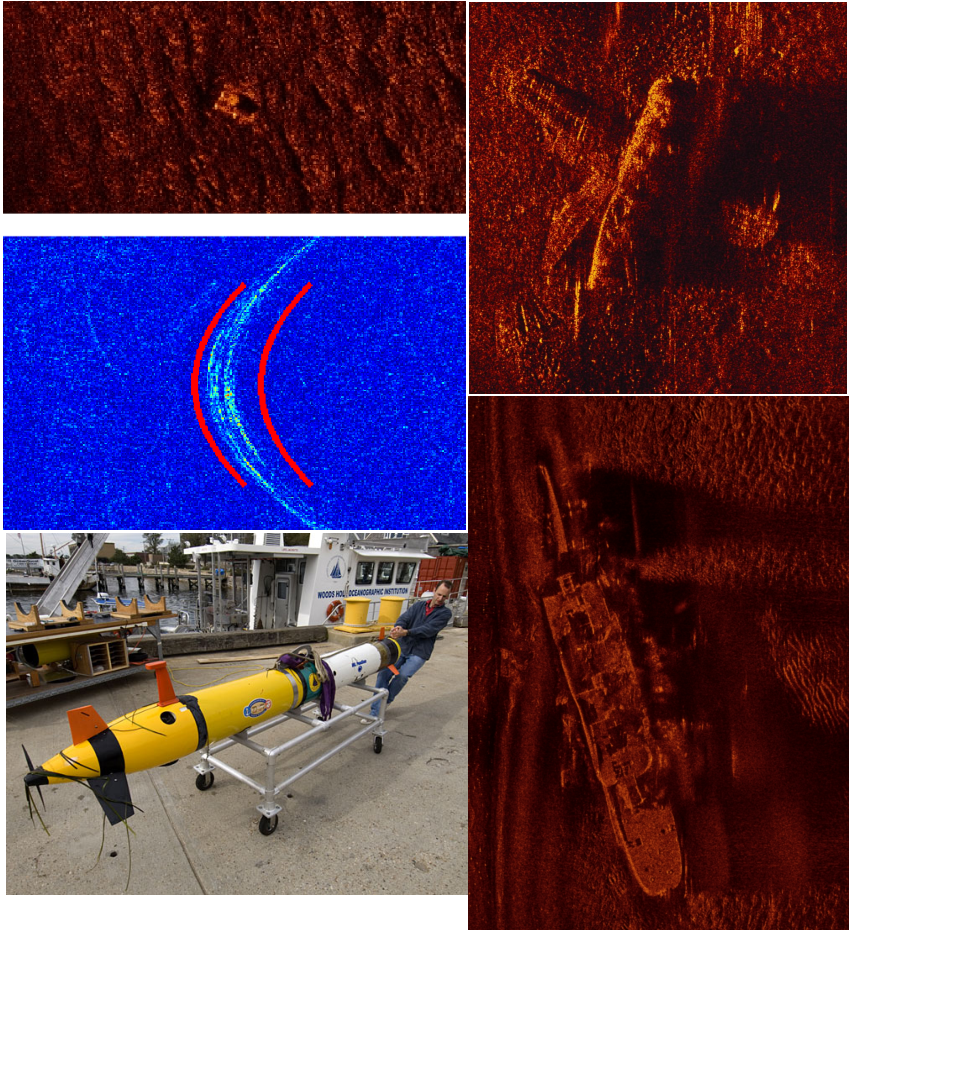
\includegraphics[scale=0.22,trim = 1 1 60 10, clip]{./projects_slide/sas.pdf}
\end{column}%
\end{columns}
\end{frame}

\begin{frame}
\frametitle{Computer Vision without Learning}
\begin{center} 
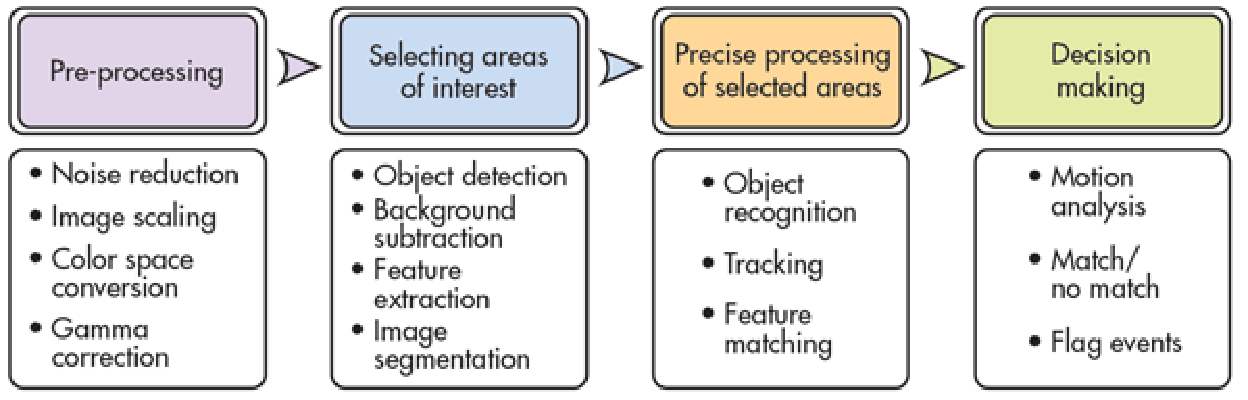
\includegraphics[scale=0.31]{./Figures/old_pipeline.pdf} \\ \vspace{0.5cm} 
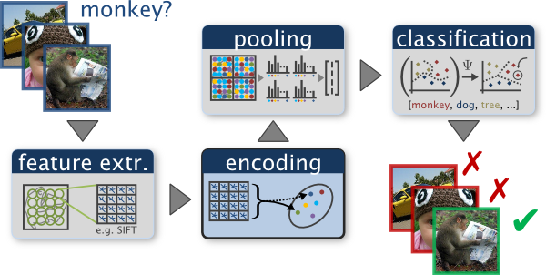
\includegraphics[scale=0.6]{./Figures/detection.pdf} \hspace{1.5cm} 
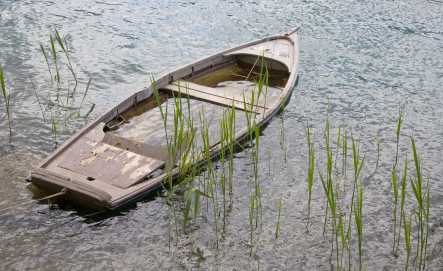
\includegraphics[scale=0.5]{./Figures/boat.jpg}\\
The engineer must manually plug all the ``leaks'' in the pipeline \\ \vspace{0.5cm} 
\tiny{http://cs.brown.edu/courses/cs143/}
\end{center} 
\end{frame} 

\begin{frame}
\frametitle{Computer Vision as of 2012}

\begin{columns}[T] % align columns
\begin{column}{.4\textwidth}
\begin{itemize} 
\item{Leverage machine learning to plug the leaks with data}
\item From engineering features $\rightarrow$ engineering \emph{feature learning architectures}   
\end{itemize} 
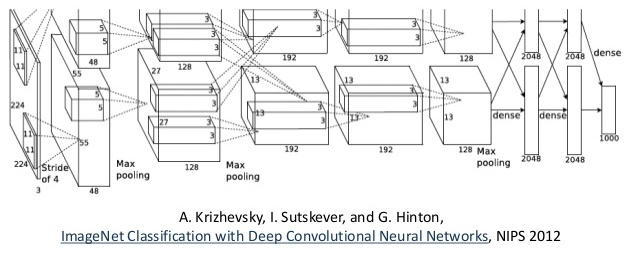
\includegraphics[scale=0.25]{./Figures/alexNet.jpg}
\end{column}%
\hfill%
\begin{column}{.6\textwidth}
\color{blue}\rule{\linewidth}{2pt}
\tiny{Tompson, Goroshin, Jain, LeCun, Bregler. \emph{CVPR 2015}}
\centering
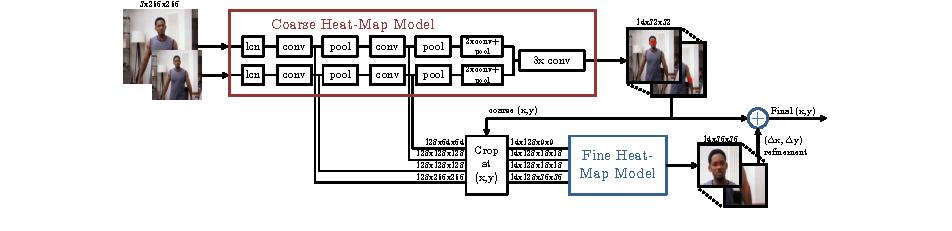
\includegraphics[scale=0.4]{./Figures/network2.pdf} \\
\tiny{Socher, Huval, Bhat, Manning, Ng. \emph{NIPS 2012}}   
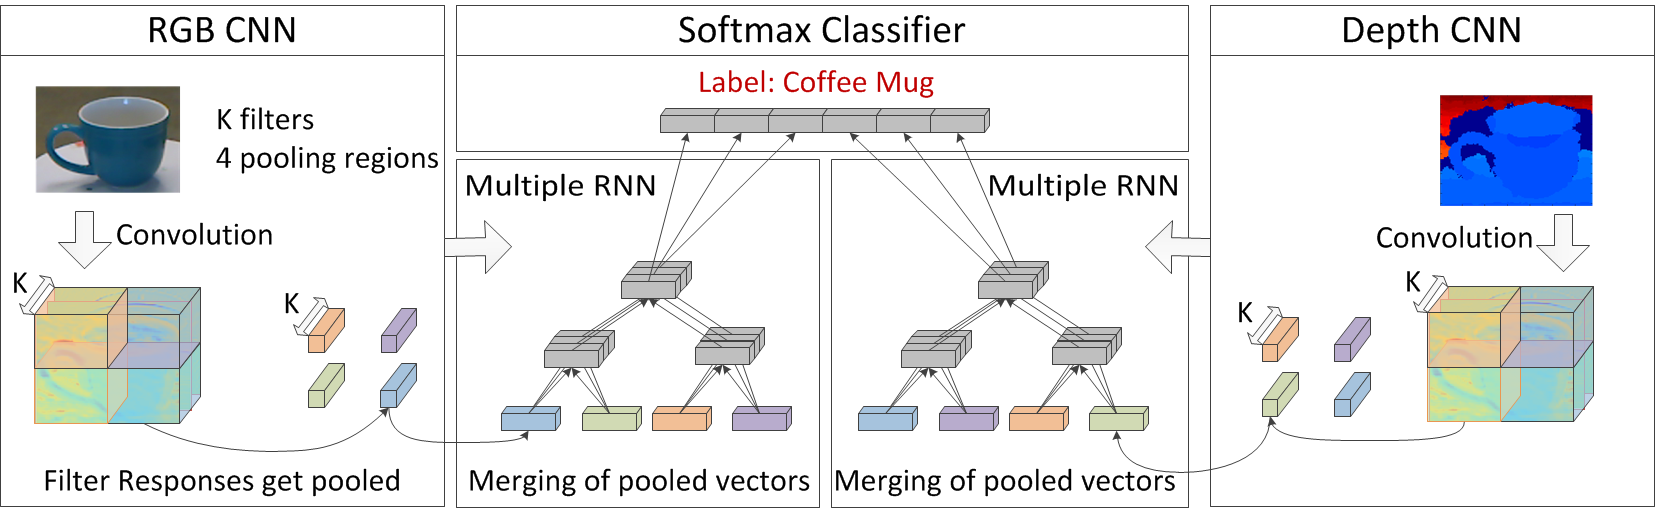
\includegraphics[scale=0.15]{./Figures/socher.png} \\
\tiny{Eigen, Puhrsch, Fergus. \emph{NIPS 2014}} \\
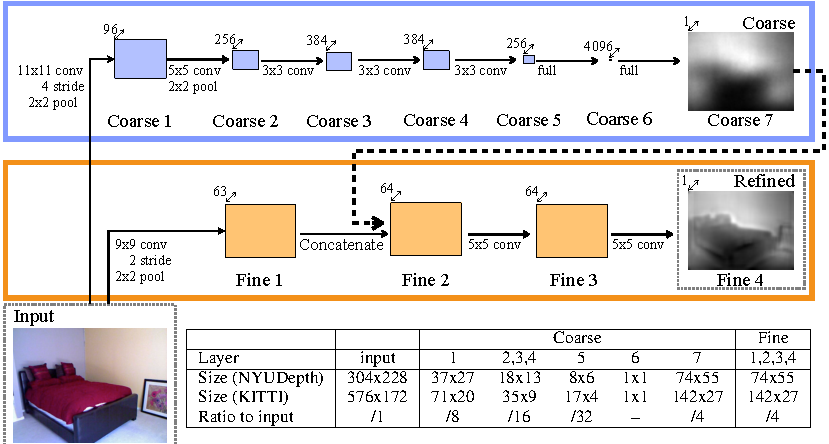
\includegraphics[scale=0.35]{./Figures/network3.pdf} \\
...and many more 
\end{column}
\end{columns}
\end{frame} 

\begin{frame}
\frametitle{Generically useful Feature Representations} 
\begin{itemize} 
\item{Experiments show that low-level features are transferable across tasks}
\item{High-level features tend to be more task-specific, i.e. the last layer must make the data linearly separable}
\item{Is there an objective that allows us to learn high-level task-agnostic representations?}
\item{Leverage virtually infinite amount of unlabeled data \bf $\rightarrow$ reduce training time, obtain better generalization, and enable on-line learning/adaptation}
\end{itemize} 
\centering
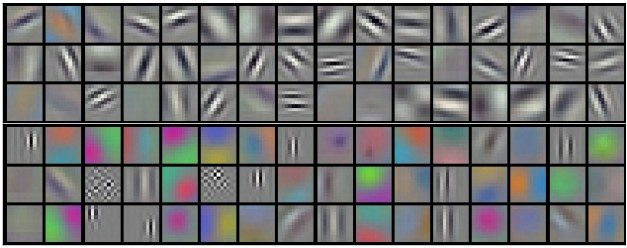
\includegraphics[scale=0.25]{./Figures/weights.jpeg} \\
\tiny{Krizhevsky et al. 2012}
\end{frame} 

\begin{frame} 
\frametitle{Representation Learning}
\end{frame} 

\end{document}



